\documentclass{article}
\usepackage[utf8]{inputenc}
\usepackage{geometry}
\usepackage{xcolor}
\usepackage{amsmath,amssymb}
\usepackage{graphicx}
\graphicspath{{./images/}}

\title{Precise vehicle localization using fusion of multiple sensors for self-driving}
\date{April 2020}
\author{ Dr. Peshala, Dr. Ranga, Chanaka, Himasha, Pasan, Ramesh}
\begin{document}
\maketitle

\section{State vector}
The state vector to be estimated is
\begin{align}
    \textbf{x} &= \left[\begin{matrix}{}\textbf{p} \\ \textbf{v} \\ \textbf{q} \\ \textbf{g} \\ \textbf{n} \\ \boldsymbol{a_b} \\ \boldsymbol{\omega_b} \end{matrix} \right]_{22\times1}
\end{align}{}
where
\begin{align}
    \textbf{p} &= (p_x, p_y, p_z) \text{ position relative to the inertial frame} \nonumber \\
    \textbf{v} &= (v_x, v_y, v_z) \text{ velocity relative to the inertial frame} \nonumber \\
    \textbf{q} &= (q_w, q_x, q_y, q_z) \text{ quaternion relative to the inertial frame} \nonumber \\
    \textbf{g} &= (g_x, g_y, g_z) \text{ gravitational vector relative to the inertial frame} \nonumber \\
    \textbf{n} &= (n_x, n_y, n_z) \text{ magnetic north vector relative to the inertial frame.} \nonumber \\
    \boldsymbol{a_b} &= (a_{bx}, a_{by}, a_{bz}) \text{ acceleration biases of the IMU} \nonumber \\
    \boldsymbol{\omega_b} &= (\omega_{bx}, \omega_{by}, \omega_{bz}) \text{ angular velocity biases of the IMU}
\end{align}{}


\section{Coordinate frames}
Following four types of coordinate frames are used.
\begin{align}
    &\mathcal{F}_{inert}=\text{ the coordinate frame fixed relative to the earth surface} \nonumber \\
    &\mathcal{F}_{gnss}=\text{ the coordinate frame in which gnss readings will be provided} \nonumber \\
    &\mathcal{F}_{body}=\text{ a coordinate frame fixed relative to the body of the vehicle} \nonumber \\
    &\mathcal{F}_{<sensor>}=\text{ coordinate frames attached to sensors in which their readings are provided} \nonumber \\
    &\text{($<sensor>$ = IMU, LiDAR etc.)}
\end{align}{}

Rotation matrix from $\mathcal{F}_{a}$ to $\mathcal{F}_{b}$ is denoted as $R_{b,a}$. Example:
\begin{align}
    \boldsymbol{r_{b}}&=R_{b,a}\boldsymbol{r_{a}}
\end{align}

\begin{figure}[htp]
    \centering
    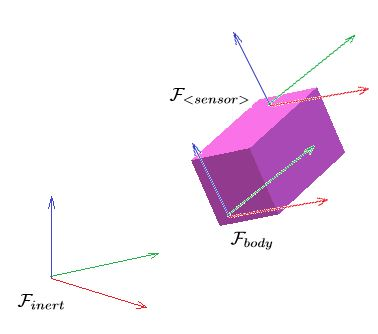
\includegraphics[width=150pt]{coordinate-frames.JPG}
    \caption{\text{Coordinate frames}}
    \label{fig-coordinate-frames}
\end{figure}

\section{Quaternion operations}
Let the unit quaternion \textbf{q} be defined as
\begin{align}
    \textbf{q} &= \left[\begin{matrix}{}q_w \\ q_x \\ q_y \\ q_z\end{matrix}\right] \\
    \text{and } \textbf{q}_v &= \left[\begin{matrix}q_x\\q_y\\q_z\end{matrix}\right]
\end{align}{}

Then some operations on \textbf{q} can be defined as given in Figure \ref{fig-quaternion-operations}.

\begin{figure}[htp]
    \centering
    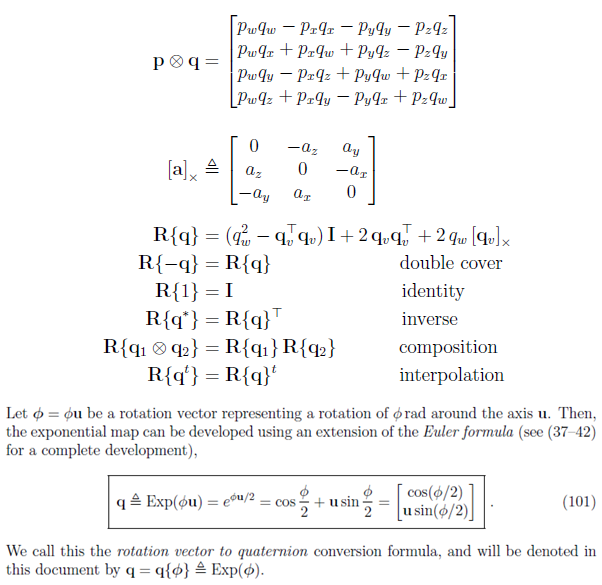
\includegraphics[width=300pt]{quaternion-operations.png}
    \caption{\text{Operations related to quaternions}}
    \label{fig-quaternion-operations}
\end{figure}








%%%%%%%%%%%%%%%%%%%%%%%%%%%%%%%%%%%%%%%%%%%%%%%%%%%%%%%%%%%%%%%%%
\section{ENU frame as the inertial frame, state vector excluding \textbf{g} and \textbf{n}}

In this approach we use,
\begin{align}
    &\mathcal{F}_{inert}=\text{East-North-Up coordinate frame with the origin at a point with precisely known GNSS} \nonumber \\
    &\quad \quad \quad  \quad \text{coordinates (considered as an inertial frame)} \nonumber \\
    &\mathcal{F}_{gnss}=\text{ WGS84 coordinate system (in lattitudes, longitudes and altitude)} \nonumber \\
    &\mathcal{F}_{body}=\text{ coordinate frame of the IMU} \text{ .}
\end{align}{}
Hence,
\begin{align}
    \mathcal{F}_{IMU}&=\mathcal{F}_{body} \text{ .}
\end{align}{}

Also the state vector is a reduced version of the original one.
\begin{align}
    \textbf{x} &= \left[\begin{matrix}{}\textbf{p}\\\textbf{v}\\\textbf{q}\\\boldsymbol{a_b}\\\boldsymbol{\omega_b}\end{matrix}\right]
\end{align}{}

\textbf{p}, \textbf{v} and \textbf{q} are expressed in $\mathcal{F}_{inert}$ frame. However the IMU biases, $\boldsymbol{a_b}$ and $\boldsymbol{\omega_b}$ are expressed in $\mathcal{F}_{body}$ frame.

\subsection{Prediction}
State updates can be given as
\begin{align}
    \Check{p}_k &= \hat{p}_{k-1}+\hat{v}_{k-1}\Delta t + \frac{1}{2} \left( R_{inert,body}\left(a_{m_{k-1}}-\hat{a}_{b_{k-1}}\right)+g\right)\Delta t^2 \\
    \Check{v}_k &= \hat{v}_{k-1}+\left(R_{inert,body}\left(a_{m_{k-1}}-\hat{a}_{b_{k-1}}\right)+g\right)\Delta t \\
    \Check{q}_k &= \hat{q}_{k-1}\otimes q\left\{\left(\omega_{m_{k-1}}-\hat{\omega}_{b_{k-1}}\right)\Delta t\right\} \\
    \Check{a}_{b_k} &= \hat{a}_{b_{k-1}} \\
    \Check{\omega}_{b_{k}} &= \hat{\omega}_{b_{k-1}}
\end{align}{}
with
\begin{align}
    R_{inert,body} &= R\left\{\hat{q}_{k-1}\right\} \text{ .}
\end{align}{}

Covariance matrix update is
\begin{align}
    \Check{\textbf{P}}_k &= F_x\hat{\textbf{P}}_{k-1}F_x^T + F_i\textbf{Q}_iF_i^T \text{ with} \\
    F_x &=\begin{array}{c|} \frac{\partial f}{\partial \delta x} \end{array}_{x_{k-1},u_{k-1}} \\
    &= \left[\begin{matrix}{}\textbf{I} & \textbf{I}\Delta t & 0 & 0 & 0 \\ 0 & \textbf{I} & -\left[R_{inert,body}\left(a_{m_{k-1}}-\hat{a}_{b_{k-1}}\right)\right]_\times\Delta t & -R_{inert,body}\Delta t & 0 \\ 0&0&\textbf{I}&0&-R_{inert,body}\Delta t \\ 0&0&0&\textbf{I}&0\\0&0&0&0&\textbf{I}\end{matrix}\right]_{15\times15} \\
    F_i &= \left[\begin{matrix}{} 0&0&0&0 \\ \textbf{I}&0&0&0 \\ 0&\textbf{I}&0&0 \\ 0&0&\textbf{I}&0 \\ 0&0&0&\textbf{I} \end{matrix}\right]_{15\times12} \\
    \textbf{Q}_i &= \left[\begin{matrix}{} \sigma_{a_n}^2\Delta t^2\textbf{I}&0&0&0 \\ 0&\sigma_{\omega_n}^2\Delta t^2\textbf{I}&0&0 \\ 0&0&\sigma_{a_\omega}^2\Delta t\textbf{I}&0 \\ 0&0&0&\sigma_{\omega_\omega}^2\Delta t\textbf{I} \end{matrix}\right]_{12\times12} \\
    \sigma_{a_n}^2 &= \text{white noise variance of IMU acceleration measurement} \\
    \sigma_{\omega_n}^2 &= \text{white noise variance of IMU angular velocity measurement} \\
    \sigma_{a_\omega}^2 &= \text{velocity random walk variance of IMU} \\
    \sigma_{\omega_\omega}^2 &= \text{angular random walk variance of IMU}
\end{align}{}

\subsection{Correction}
Steps for correction upon receiving a measurement can be given as follows.
\begin{align}
    K_k &= \Check{\textbf{P}}_kH^T\left(H\Check{\textbf{P}}_kH^T+V\right)^{-1} \\
    \hat{\textbf{P}}_k &= \left(\textbf{I}-K_kH\right)\Check{\textbf{P}}_k
\end{align}{}
Here,
\begin{align}
    H &= H_xX_{\delta x} \text{ and} \\
    X_{\delta x} &= \left[\begin{matrix}{}\textbf{I}&0&0&0&0\\0&\textbf{I}&0&0&0\\0&0&Q_{\delta \theta}&0&0\\0&0&0&\textbf{I}&0\\0&0&0&0&\textbf{I}\end{matrix}\right]_{16\times15} \\
    Q_{\delta\theta} &=\frac{1}{2} \left[\begin{matrix}{}-q_x&-q_y&-q_z\\q_w&q_z&-q_y\\-q_z&q_w&q_x\\q_y&-q_x&q_w\end{matrix}\right]_{4\times3}
\end{align}{}

For a GNSS measurement where position is measured relative to $\mathcal{F}_{inert}$ in all three directions,
\begin{align}
    H_x &= \left[\begin{matrix}{}\textbf{I}&0&0&0&0\end{matrix}\right]_{3\times16} \text{ and} \\
    \Hat{\delta x}_k &= K_k\left(y-\Check{p}_k\right)
\end{align}{}

Steps for injecting the error to the state are as follows.
\begin{align}
    \hat{p}_k &= \Check{p}_k + \hat{\delta p}_k \\
    \hat{v}_k &= \Check{v}_k + \hat{\delta v}_k \\
    \hat{q}_k &= q\left\{\hat{\delta\theta}_k\right\}\otimes\Check{q}_k \\
    \hat{a_b}_k &= \Check{a_b}_k + \hat{\delta a_b}_k \\
    \hat{\omega_b}_k &= \Check{\omega_b}_k + \hat{\delta \omega_b}_k \\
\end{align}{}

Finally the error state is reset to zero ($\boldsymbol{\delta x}\xleftarrow{}0$).

\subsection{Initialization}
\begin{align}
    \boldsymbol{\delta x} &= \textbf{0} \\
    p_0 &= \text{GNSS position of the starting point expressed in $\mathcal{F}_{inert}$ frame.} \\
    v_0 &= 0 \\
    q_0 &= \text{Orientation determined by the gravity and magnetic North vectors.} \\
    a_{b_0},\omega_{b_0} &= \text{given in datasheet of the IMU/ previous estimate.} \\
    g &= \left(0,0,-9.8\right)
\end{align}{}

\subsection{Orientation from magnetic field vector}
Let the normalized magnetic field and gravitational vectors in $\mathcal{F}_{inert}$ frame be $m_i$ and $g_i$. Then
\begin{align}
    m_i &= \left[\begin{matrix}0 & -1 & 0 \end{matrix}\right]^T \text{ and} \\
    g_i &= \left[\begin{matrix}0 & 0 & -1\end{matrix}\right]^T \text{ .}
\end{align}
Let the unit quaternion corresponding to the orientation of the vehicle be $q = \left[\begin{matrix}w & x & y & z\end{matrix}\right]^T$ and $R_{inert,body} = R_{inert,body}\left\{q\right\}\left(\text{Rotation matrix corresponding to }q\right)$. If the measured, normalized magnetic field and acceleration vectors in $\mathcal{F}_{IMU} = \mathcal{F}_{body}$ are given by $m_s = \left[\begin{matrix}m_x&m_y&m_z\end{matrix}\right]^T$ and $f_s = \left[\begin{matrix}f_x&f_y&f_z\end{matrix}\right]^T$, when the vehicle is at rest we can have the following set of equations.
\begin{align}
    R_{inert,body}\cdot m_s + m_i &= 0 \\
    R_{inert,body}\cdot f_s + g_i &= 0 \\
    w^2+x^2+y^2+z^2 -1 &= 0
\end{align}
The quaternion components are approximated by fitting a least-square-error line for the above set of over-determined non-linear equations. Furthermore, since the accelerometer reading is much reliable than the magnetometer reading, the orthogonality of the gravity and magnetic filed vectors can be utilized apply a correction to the magnetic field vector. In the following approach, we expect to remove any magnetic field components in the direction parallel to that of gravity. Let $m_s^{raw}$ and $f_s^{raw}$ be the raw magnetic field and acceleration vectors measured by the sensor at rest and $m_s$ be the corrected, normalized magnetic field vector.
\begin{align}
    m'_s &= m_s^{raw} - (m_s^{raw} \cdot f_s^{raw}) \frac{f_s^{raw}}{||f_s^{raw}||^2} \\
    m_s &= \frac{m'_s}{||m'_s||}
\end{align}



%%%%%%%%%%%%%%%%%%%%%%%%%%%%%%%%%%%%%%%%%%%%%%%%%%%%%%%%%%%%%%%%%
\section{Initial body frame as inertial frame, full state vector}

In this approach we use,
\begin{align}
    &\mathcal{F}_{inert}=\text{a coordinate frame with axes parallel to those of the IMU frame at the initialization, and} \nonumber \\
    &\quad \text{the origin at a point with precisely known GNSS coordinates (considered as an inertial frame)} \nonumber \\
    &\mathcal{F}_{gnss}=\text{ WGS84 coordinate system} \nonumber \\
    &\mathcal{F}_{body}=\text{ coordinate frame of the IMU} \text{ .}
\end{align}{}
Hence,
\begin{align}
    \mathcal{F}_{IMU}&=\mathcal{F}_{body} \text{ .}
\end{align}{}

\textbf{p}, \textbf{v}, \textbf{q}, \textbf{g} and \textbf{n} are expressed in $\mathcal{F}_{inert}$ frame. However the IMU biases, $\boldsymbol{a_b}$ and $\boldsymbol{\omega_b}$ are expressed in $\mathcal{F}_{body}$ frame.

State vectors are initialized in the following manner.
\begin{align}
    \textbf{p}&=\text{initial GNSS reading converted to }\mathcal{F}_{inert} = C_{inert,gnss}\left(\boldsymbol{y}\ominus\boldsymbol{y_0}\right) \\
    \textbf{v}&=\left(0,0,0\right) \\
    \textbf{q}&=\left(0,0,0\right)\\
    \textbf{g}&=\text{initial true acceleration due to gravity measured by the IMU} \\
    \textbf{n}&=\text{North vector calculated using the initial reading of the magnetometer} \\
    \boldsymbol{a_b},\boldsymbol{\omega_b}&=\text{from data given by the manufacturer/ previous estimate, if available}
\end{align}{}
Here, $\boldsymbol{y}$ is the GNSS reading at the starting point and $\boldsymbol{y_0}$ is the GNSS coordinate of the origin of $\mathcal{F}_{inert}$. Note that $C_{inert,gnss}$ (and therefore $C_{gnss,inert}$) depends on \textbf{g} and \textbf{n}.



%%%%%%%%%%%%%%%%%%%%%%%%%%%%%%%%%%%%%%%%%%%%%%%%%%%%%%%%%%%%%%%%%
\section{GNSS measurement auto-regressive model}
As the GNSS measurement error (with respect to the ground truth) shows non-zero higher order correlations, it is modeled as a first order auto-regressive process [Zui Tao. Autonomous road vehicles localization using satellites, lane markings and vision, 2016]. Let the GNSS measurement, ground truth and the gnss error at time $k$ be $x_k,\hat{x}_k \text{ and }e_k$ respectively. Then,
\begin{align}
    e_{k+1} &= a_1e_k + \omega_{k+1} \\
    (x_{k+1}-\hat{x}_{k+1}) &= a_1(x_k-\hat{x}_k) + \omega_{k+1} \\
    \hat{x}_{k+1} &= x_{k+1} - a_1(x_k-\hat{x}_k)-\omega_{k+1}
\end{align}
Here, $\omega_{k}$ is a gaussian white noise term with variance equal to that of the receiver. Although, in the above mentioned paper, they are using a separate states for estimating the GNSS error terms, we intend to simply calculate the parameters ($a_1$) using statistical methods and use the above result to generate a corrected version (with zero correlation) of the measurement. 




%%%%%%%%%%%%%%%%%%%%%%%%%%%%%%%%%%%%%%%%%%%%%%%%%%%%%%%%%%%%%%%%%
\section{KAIST Urban dataset}



\end{document}

